\documentclass[conference]{IEEEtran}
\usepackage[utf8]{inputenc}
\usepackage[pdftex]{hyperref}
\usepackage{algorithmic}
\usepackage{cite}
\usepackage{graphicx}

% correct bad hyphenation here
\hyphenation{op-tical net-works}


\begin{document}

\title{A proximity localization system for routing audio streams based on Bluetooth technology}
\author{Davide~Pesavento, Martina~Astegno \\
	Università degli Studi di Padova \\
	Corso di Laurea Magistrale in Informatica \\
	\{dpesaven,mastegno\}@studenti.math.unipd.it
}
%\author{\IEEEauthorblockN{Davide Pesavento}
%\IEEEauthorblockA{Universit\`{a} degli Studi di Padova\\
%Corso di Laurea Magistrale in Informatica\\
%Email: email@studenti.math.unipd.it}
%\and
%\IEEEauthorblockN{Martina Astegno}
%\IEEEauthorblockA{Universit\`{a} degli Studi di Padova\\
%Corso di Laurea Magistrale in Informatica\\
%Email: martina.astegno@studenti.unipd.it}}

\maketitle

\begin{abstract}
In this paper we present a prototype application that shows how the Bluetooth technology can be used to locate a person wearing a Bluetooth device (e.g. a smartphone) among a set of rooms. The final aim is to playback an audio stream stored in a central server and move it from a speaker to another, situated in every room, following the person's movements.
\end{abstract}

\begin{IEEEkeywords} % normally used for peerreview paper
Bluetooth, BlueZ, DBus, PulseAudio, audio routing, smartphone.
\end{IEEEkeywords}


% For peer review papers, you can put extra information on the cover
% page as needed:
% \ifCLASSOPTIONpeerreview
% \begin{center} \bfseries EDICS Category: 3-BBND \end{center}
% \fi
%
% For peerreview papers, this IEEEtran command inserts a page break and
% creates the second title. It will be ignored for other modes.
\IEEEpeerreviewmaketitle


%\hfill October 16, 2010

\section{Introduction}
\subsection{Bluetooth technology}
Bluetooth is an open specification for a radio system that provides the network infrastructure to enable short range wireless communication of data and voice. It comprises of a hardware component and a software component. The specification also describes usage models and user profiles for these models.
Bluetooth supports two kinds of links: Asynchronous Connectionless (ACL) links for data transmission and Synchronous Connection Oriented (SCO) links for audio/voice transmission. It uses Frequency Hopping Spread Spectrum (FHSS) to avoid any interference. A Bluetooth channel is divided into time slots each 625 micro second in length. The devices hop through these timeslots making 1600 hops per second. This trades bandwidth efficiency for reliability, integrity and security.
In figure \ref{stack} we can see the architecture of Bluetooth protocol.\\
\begin{figure}[h]
\centering
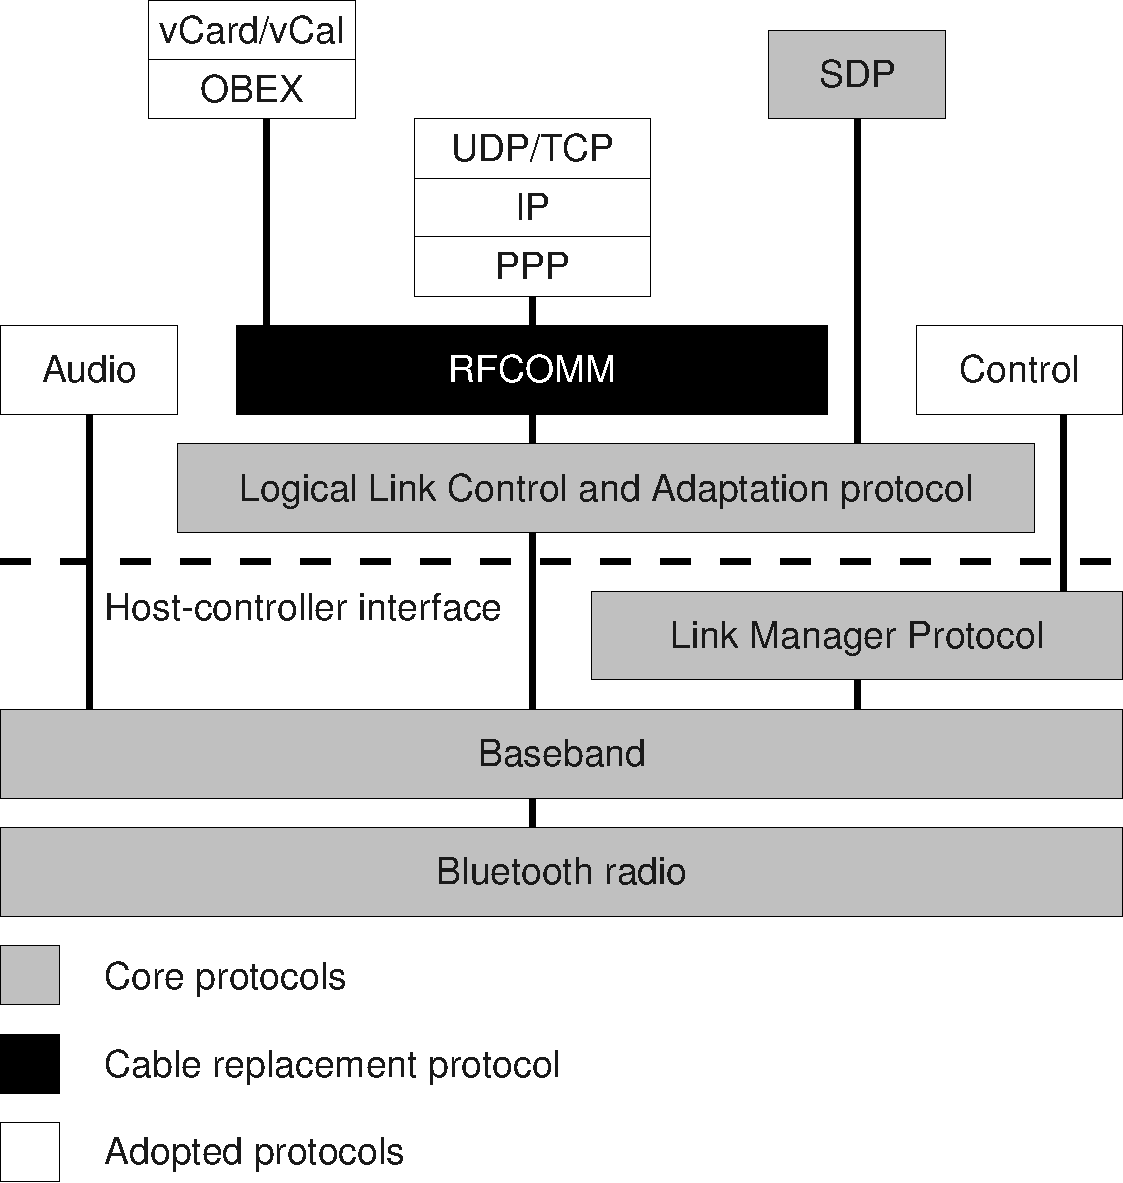
\includegraphics[scale = 0.3]{BTstack.pdf}
\caption{Bluetooth protocol stack}
\label{stack}
\end{figure}
In our project we adopt a specific Bluetooth stack implementation, \textbf{Bluez} version 4 or later, that provides support for the core Bluetooth layers and protocols. It is flexible, efficient and uses a modular implementation. \\

Current versions of BlueZ consist of many separate modules:
\begin{itemize}
\item Bluetooth kernel subsystem core
\item L2CAP and SCO audio kernel layers
\item RFCOMM, BNEP, CMTP and HIDP kernel implementations
\item HCI UART, USB, PCMCIA and virtual device drivers
\item General Bluetooth and SDP libraries and daemons
\item Configuration and testing utilities
\item Protocol decoding and analysis tools
\end{itemize}




\subsection{PulseAudio Server}
PulseAudio is a sound server for POSIX and Win32 systems. A sound server is basically a proxy for sound applications. It allows to do advanced operations on sound data as it passes between an application and the hardware. Things like transferring the audio to a different machine, changing the sample format or channel count and mixing several sounds into one are easily achieved using a sound server. In this context the main functionalities used are the audio stream control, to transfer the sound between different speakers according to the person movement and the simoultaneously playback from two or more speakers.

\section{General architecture}

\subsection{Requirements}
Before detailing the design of the prototype, we would like to point out some basic requirements for the project. Here, we propose a list and a description for the main ones.
\begin{itemize}
\item{\textbf{Smartphone}:} the device used to determine the room in which the person is. We will assume that there is only one smartphone.
\item{\textbf{Central server}:} it runs the main application and controls all the communications from/to the Bluetooth adapters.
\end{itemize}
Inside each room there must be available:
\begin{itemize}
\item{a \textbf{Bluetooth adapter}:} it detects the received signal strength (RSSI) and sends it to the server through a very simple command-line application;
\item{a \textbf{speaker}:} it lets out sound when the associate Bluetooth adapter is selected for playback.
\end{itemize}


\subsection{Bluetooth module}
The main component of the system is the Bluetooth module, that manages the RSSI values and communications between Bluetooth hosts and device. It is based on a simple and efficient application, named \texttt{probe} and associated to every Bluetooth adapter, that is able to interface with \textbf{BlueZ} through \textbf{DBus}. In detail, every Bluetooth adapter is modeled by the class \texttt{ProbeInterface}, that allows to start and stop a discovery done by the device and to update the RSSI values when a change occurs. All \texttt{ProbeInterface} objects are controlled by the class \texttt{ProbeManager} that monitors the device localization and stores the information about every \texttt{ProbeInterface} (e.g. the room name associated with the adapter).

\subsection{Pulseaudio module}
The PulseAudio daemon exposes two data structures in which our application is interested.
\begin{itemize}
\item \texttt{pa\_sink}:
\item \texttt{pa\_sink\_input}:
\end{itemize}

To control and monitor the PulseAudio operations we implemented the class \texttt{PAController}. There are three main methods:
\begin{itemize}
\item \texttt{PAController::createTunnel(QByteArray)}
\item \texttt{PAController::moveSinkInput(SinkInput, QList<QByteArray>)}
\item \texttt{PAController::combineTunnels(QList<QByteArray>, QString, int, QString}
\end{itemize}
The first method allows to create a sink that acts as tunnel connection with the server specified in the parameter in which it's running a PulseAudio daemon. This operation is done loading a particular module called \texttt{module-tunnel-sink}. When it's available the complete list of sinks, we can redirect the \texttt{pa\_sink\_input} coming from a specific application (e.g. MPlayer) to one or more sinks associated with a speaker in each room. In detail to realize this movement we implemented the second method, \texttt{moveSinkInput()}, that redirects the \texttt{SinkInput} specified in this first parameter to the speakers contained in the second one.
By default the audio is reproduced by only one \texttt{pa\_sink}. With the third method it is possible to playback sound through more speakers simultaneously, loading the PulseAudio \texttt{module-combine} that combines more objects \texttt{pa\_sink} creating a new sink with a specified identifier.


\subsection{Algorithm}
The implemented algorithm chooses which speaker has to playback sound according to person's location; we can suppose infact that the signal power detected by the Bluetooth adapter is higher than the other RSSI values in the room where person is situated. The following pseudo-code shows how the algorithm works. The output returned represents the index of speakers/rooms where the sound has to be reproduced.

Input variables:
\begin{itemize}
\item \textbf{retryCount}: the time spent from inizialization to the request of available RSSIs.
\item \textbf{maxRetries}: the threshold that when exceeded the playback is forced to start, even if there aren't all data available.
%\item \textbf{sortedRssi}: the map with every devices, sorted by the RSSI value associated with each ones.
\item \textbf{curRooms}: it's a set that contains the addresses of rooms in which the playback occurs in the current moment.
%\item \textbf{No\_null\_RSSI}: number of available RSSI values.
\item \textbf{adjacencyMap}: the map stores the list of adjoining rooms for every specific room.
\item \textbf{rssiMap}: it stores for every Bluetooth adapter the RSSI value detected.
%\item \textbf{minNumberRssi}: min number of RSSI required to proceed with the sound playback.
\item \textbf{maxSimultaneousSpeakers}: max number of speakers that can be activated simultanously.
\end{itemize}
\textbf{\underline{ChooseOutputs algorithm:}}
\vspace{0.3cm}
\begin{algorithmic}[1]

\STATE $outputs \gets null$ \COMMENT{Create the variable to return the list of speakers to activate for playback}
\STATE $retryCount \gets 0$
\STATE $sort$ $(rssiMap)$ \COMMENT{Sort the RSSI values}

\STATE $results \gets null$
\FOR{$i = 1$ to $ maxSimultaneouslySpeakers$}
\STATE $results \gets results$ $\cup$ $rssiMap$ $(i)$ \COMMENT{Choose the rooms with highest RSSI with UB and insert them into $results$}
\ENDFOR

\IF{($results$ is empty) \textbf{and} ($retryCount < maxRetries$)}
\STATE $ retryCount \gets retryCount + 1 $ \COMMENT{Wait a bit more if we don't have enough data}
\STATE GOTO 3)
\ENDIF

\FOR{$i = 1$ to $ numElements$ $(results)$}
	\IF{$ results(i) \in adjacencyMap$ $(curRooms)$}
		\STATE $outputs \gets outputs$ $\cup$ $results(i)$ \COMMENT{Add element after intersection with rooms contiguous to the current ones}
	\ENDIF
\ENDFOR
\RETURN outputs
\end{algorithmic}
%In the algorithm just exposed the method \texttt{add(Object[] param1, Object param2)} symple adds \texttt{param2} to the list contains in \texttt{param1}.

%\subsection{Tester}
%bisogna mettere che i dati sono precompilati, perchè non avevamo l'HW adatto che fornisse i lvalore di RSSI in seguito a d una inquiry.

\section{How the system work}
\begin{figure}[h]
\centering
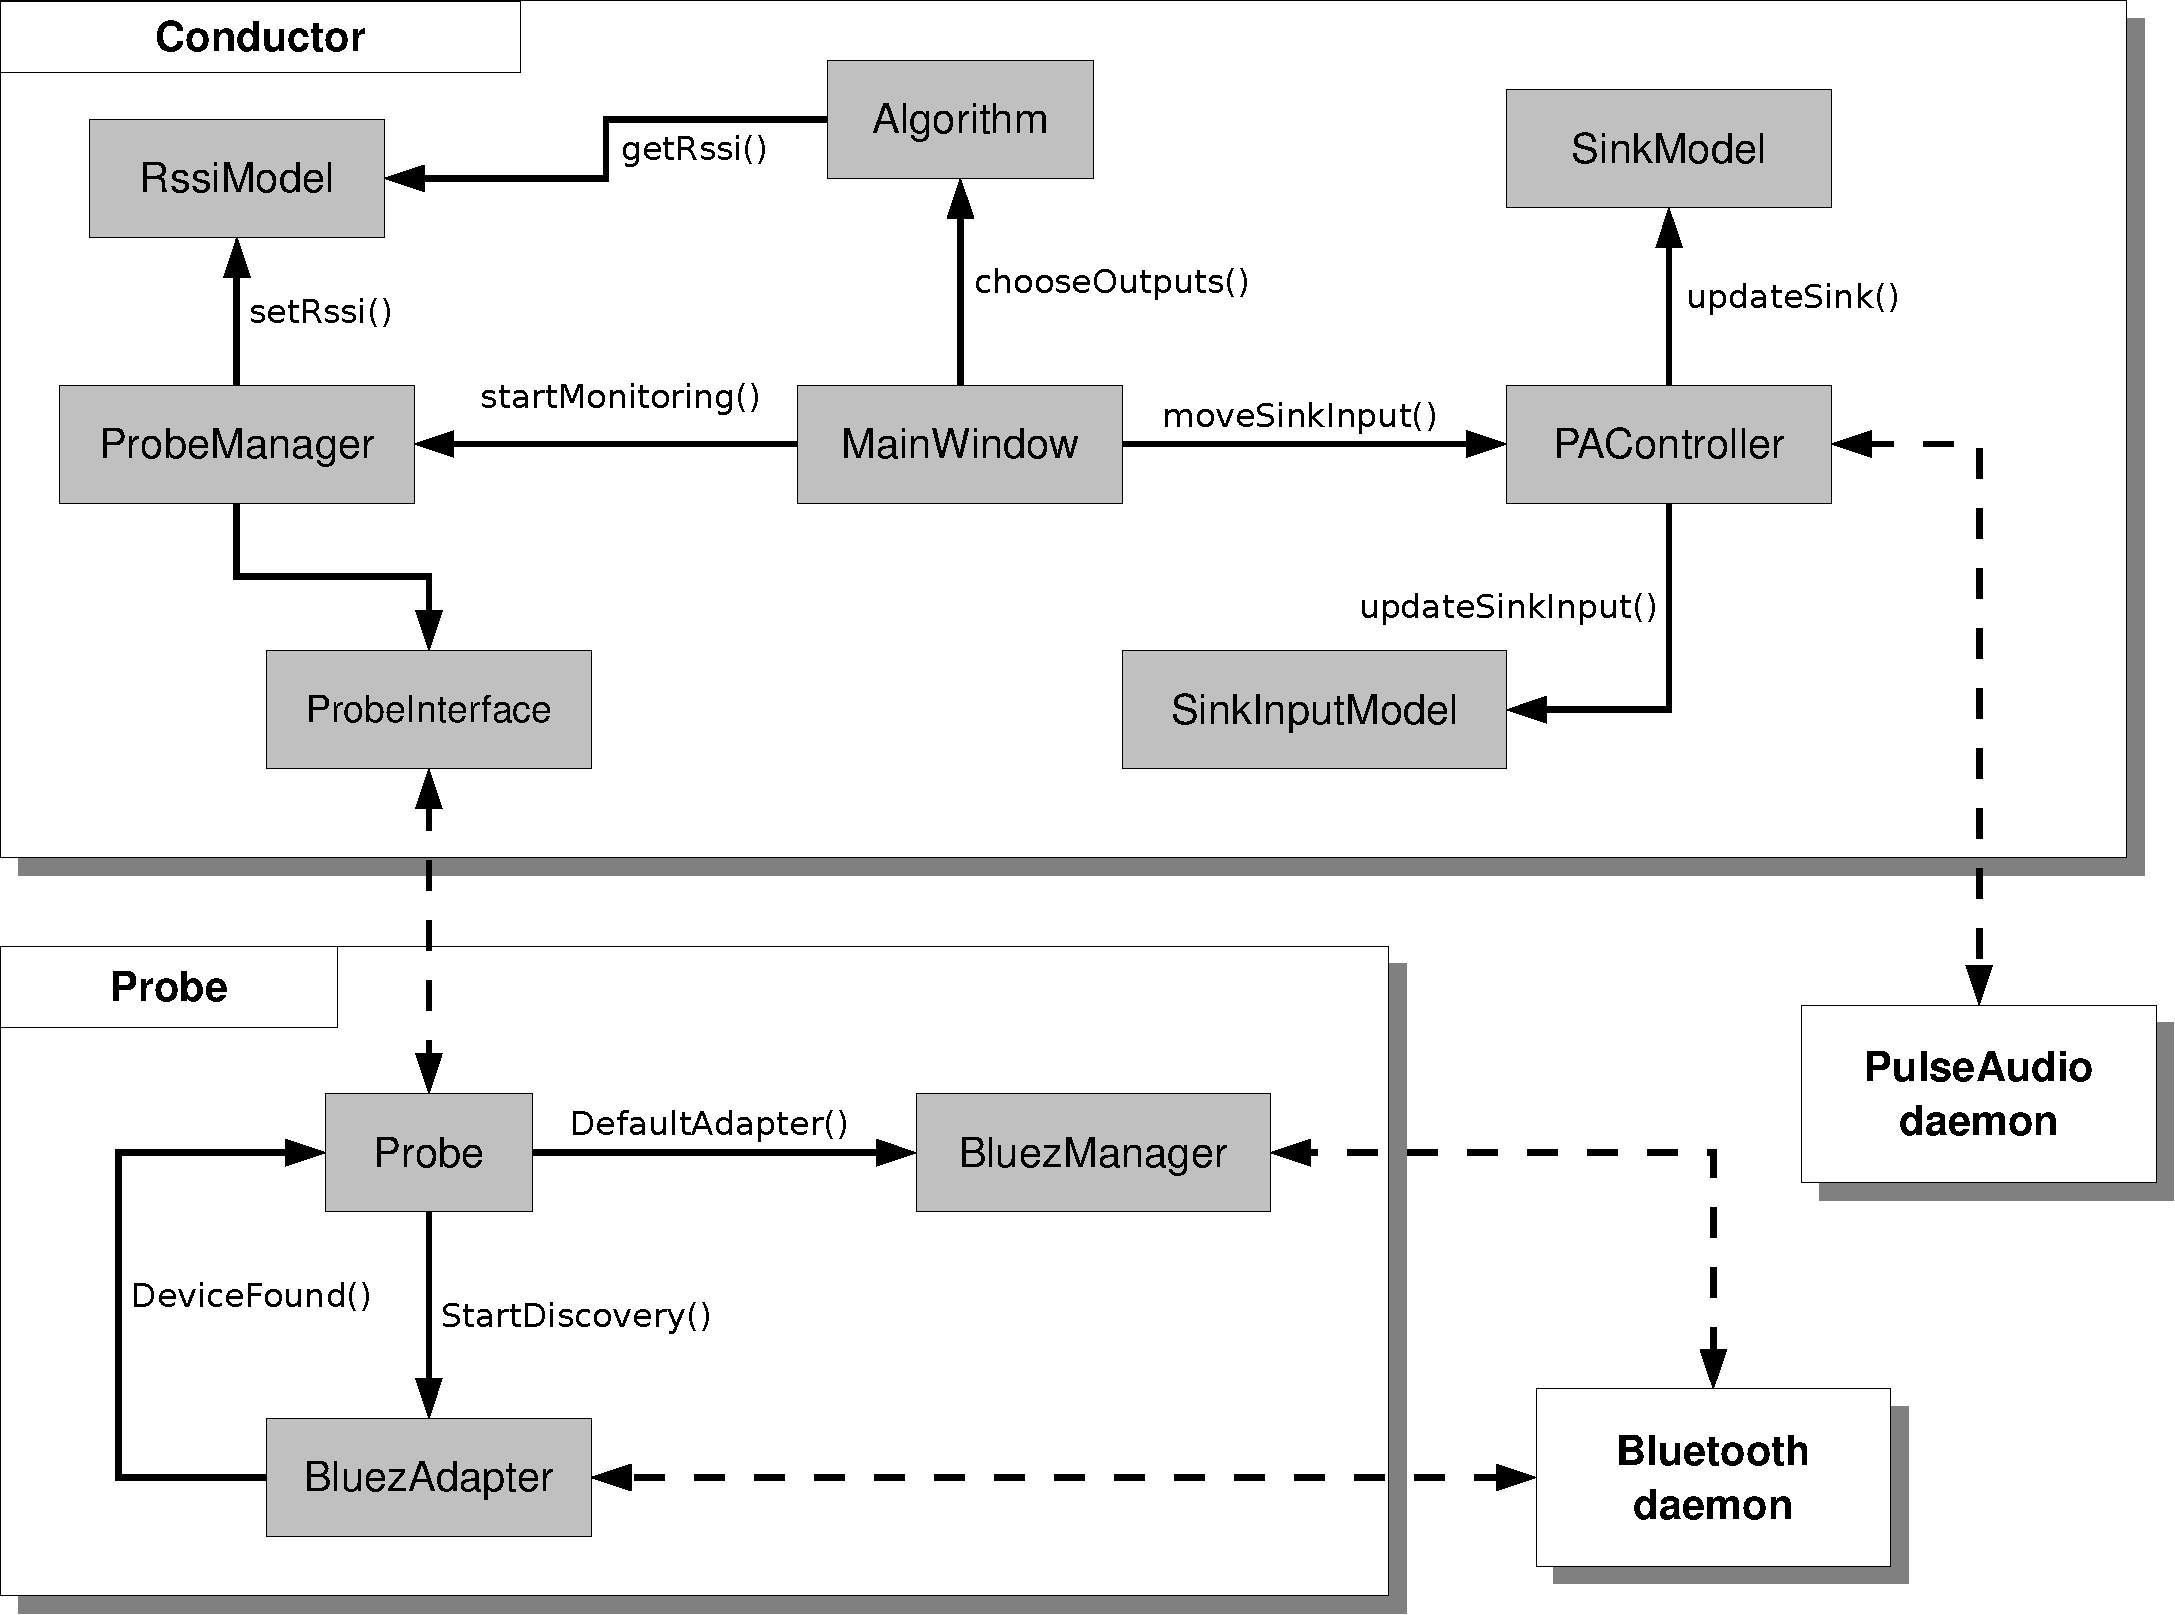
\includegraphics[scale = 0.3]{architettura.pdf}
\caption{Interaction between components}
\label{arch}
\end{figure}

\subsection{Configuration}
Before starting the application it is necessary to setup some parameters in the configuration file. The information to provide are:
\begin{itemize}
\item \texttt{maxRetries}: it represents a threshold. When crossed the playback is forced to start.
\item \texttt{maxSimultaneousSpeakers}: the max number of speakers activated at the same time.
\item \texttt{probesAddresses}: the IP addresses of Probes associated with each room.
\item \texttt{roomsNames}: the names associated with each room.
\item \texttt{roomsTopology}: it describes the relative localization of each room. %respect to each other.
\item \texttt{updateInterval}: it represents the time interval (in milliseconds) the algorithm is executed. 
\end{itemize}

\subsection{Runtime behavior}
%description about components interaction
In this section we will describe the system runtime behavior, showing how different components can interact and how the RSSI values are used to control the audio stream.
Periodically, through an inquiry, the Probes will obtain the RSSI values detected with respect the smartphone. If the difference between the new and the preceeding RSSI values is higher than a fixed threshold, the Probes transmit them to the main application on the central server. This operation is executed at regular intervals to estimate in which room the person with the device is. If this is different from the room in which the playback is currently running, this information is comunicated to the \texttt{PAController} and a request is sent to move the selected audio stream to the speaker associated with the new room. At this point there are two possible scenarios according to the number of speakers that have to be activated:
\begin{itemize}
\item one speaker: the audio stream is directly redirected to the respective tunnel;
\item two or more speakers: it is necessary to load the combine-module (Pulseaudio module), that creates a virtual sink to reproduce the stream through all the connected sinks (slaves).
\end{itemize}

\section{Experiments Evaluation}

\section{Future work and conclusion}
Here we will explain some possible project extensions.
\subsection{Improve testing phase}
Currently our application has been tested using an additional component that simulates the person movements. In detail it is a particular interface (a button) associated with each Probe application. By clicking it we can increase the RSSI value associated with the respective adapter and consequently decrease the RSSI values associated with the other adapters. However being only a simulation, the behavior doesn't totally match  with the real one. To improve the coherence and the reliability of test results it should use an hardware with specific requirements. It should arrange for each rooms, in the apartment, a Bluetooth adapter that should be able to reply to an inquiry request providing the RSSI value detected. So with the complete list of RSSI it is possible to run the algorithm with true values and choose where the playback can start.
\subsection{Multiple devices}
Although an assumption of the present project is the identification of a single smartphone, it would be important to allow the application to support and manage multiple devices. This entails the necessity to consider how different devices could interact and interfere between them.
\subsection{``Mixer'': application on device}
In our project the main application runs in the central server and the device (smartphone) is only used to localize the person. It would be interesting to develop an application for the smartphone to give the user a certain control on the audio stream. For instance with this new feature the person should be able to regulate the volume and to stop the playback. A further improvement could be an interface to navigate through the playlist, i.e. choose a specific song or skip to the previous/next track.


\begin{thebibliography}{1}
\bibitem{Pulseaudio}
		PulseAudio Sound Server,
		\url{http://www.pulseaudio.org/}
\bibitem{PulseaudioDoc}
		PulseAudio documentation
		\url{http://0pointer.de/lennart/projects/pulseaudio/doxygen/}
\bibitem{Bluez}
		BlueZ: official Linux Bluetooth protocol stack,
		\url{http://www.bluez.org/}

\end{thebibliography}

\end{document}
